\documentclass[border=0pt]{standalone}
\usepackage{tikz}
\usepackage{amsmath, amsthm, amssymb}
%\input{commondefinitions}
\usetikzlibrary{plotmarks}
\newcommand\marksymbol[2]{\tikz[#2,scale=1.2]\pgfuseplotmark{#1};}

\colorlet{coscolor}{blue}
\newcommand{\cuadritotikz}{
% \pgfmathsetmacro{\unitstep}{5.2}
% \node at (-0.5,0.5) {(a)} ;
    \foreach \x in {0,1,2,3} {
      \foreach \y in {0,1,2,3} {
        \begin{scope}[shift={(\x,-\y)}] 
          \draw[black!10] (0,0) rectangle (1,1); 
%           \node at (0.5,0.5) {$\tau_{\y,\x}$};
         \end{scope}
%         \node[block] at (2,-\y) (block\y) {$f_\y$};
%         \draw[->] (block\y.east) -- +(0.5,0);
    }
    }
 \draw (0,-3) rectangle (4,1);
}

\begin{document}
\pagestyle{empty}
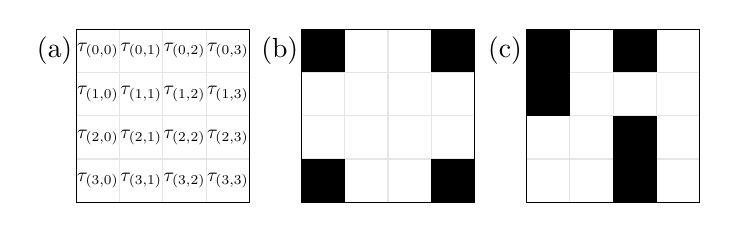
\begin{tikzpicture}[x=0.55cm, y=0.55cm] % {{{
\pgfmathsetmacro{\unitstep}{5.2}
\begin{scope}[shift={(0*\unitstep,0)}] % Coordenadas {{{
\node at (-0.5,0.5) {(a)} ;
% \cuadritotikz{}
    \foreach \x in {0,1,2,3} {
      \foreach \y in {0,1,2,3} {
        \begin{scope}[shift={(\x,-\y)}] 
          \draw[black!10] (0,0) rectangle (1,1); 
%           \draw (0,0) rectangle (1,1); 
          \node at (0.5,0.5) {\scalebox{.7}{$\tau_{(\y,\x)}$}};
         \end{scope}
%         \node at (0,-\y) (input\y) {$i_\y$};
%         \node[block] at (2,-\y) (block\y) {$f_\y$};
%         \draw[->] (input\y) -- (block\y);
%         \draw[->] (block\y.east) -- +(0.5,0);
    }
    }
 \draw (0,-3) rectangle (4,1);
\end{scope} % }}}
\begin{scope}[shift={(1*\unitstep,0)}] % Good channel {{{
\node at (-0.5,0.5) {(b)} ;
\cuadritotikz{}
%     \foreach \x in {0,1,2,3} {
%       \foreach \y in {0,1,2,3} {
%         \begin{scope}[shift={(\x,-\y)}] 
%           \draw (0,0) rectangle (1,1); 
% %           \node at (0.5,0.5) {$\tau_{\y,\x}$};
%          \end{scope}
% %         \node at (0,-\y) (input\y) {$i_\y$};
% %         \node[block] at (2,-\y) (block\y) {$f_\y$};
% %         \draw[->] (input\y) -- (block\y);
% %         \draw[->] (block\y.east) -- +(0.5,0);
%     }
%     }
\begin{scope}[shift={(0,-3)}] \fill[black] (0,0) rectangle (1,1); \end{scope}
\begin{scope}[shift={(3,-3)}] \fill[black] (0,0) rectangle (1,1); \end{scope}
\begin{scope}[shift={(0,0)}] \fill[black] (0,0) rectangle (1,1); \end{scope}
\begin{scope}[shift={(3,0)}] \fill[black] (0,0) rectangle (1,1); \end{scope}
\end{scope} % }}}
\begin{scope}[shift={(2*\unitstep,0)}] % Good channel {{{
\node at (-0.5,0.5) {(c)} ;
\cuadritotikz{}
%     \foreach \x in {0,1,2,3} {
%       \foreach \y in {0,1,2,3} {
%         \begin{scope}[shift={(\x,-\y)}] 
%           \draw (0,0) rectangle (1,1); 
% %           \node at (0.5,0.5) {$\tau_{\y,\x}$};
%          \end{scope}
% %         \node at (0,-\y) (input\y) {$i_\y$};
% %         \node[block] at (2,-\y) (block\y) {$f_\y$};
% %         \draw[->] (input\y) -- (block\y);
% %         \draw[->] (block\y.east) -- +(0.5,0);
%     }
%     }
\begin{scope}[shift={(0,0)}] \fill[black] (0,0) rectangle (1,1); \end{scope}
\begin{scope}[shift={(0,-1)}] \fill[black] (0,0) rectangle (1,1); \end{scope}
\begin{scope}[shift={(2,0)}] \fill[black] (0,0) rectangle (1,1); \end{scope}
\begin{scope}[shift={(2,-2)}] \fill[black] (0,0) rectangle (1,1); \end{scope}
\begin{scope}[shift={(2,-3)}] \fill[black] (0,0) rectangle (1,1); \end{scope}
\end{scope} % }}}
\end{tikzpicture} % }}}
\end{document}
